\chapter{Results}
\label{chap:results}


\section{Hyperparameter gridsearch}

The extended search grid for the hyperparameters of the retrained SMILES models, along with the results from the gridsearch of MassSpecGym, can be found in table \ref{tab:gridsearch}.
The hyperparameter combination for which the trained model has lowest validation loss is denoted in bold.

\begin{table}[h]
	\caption{
		SMILES transformer, Gridsearch MassSpecGym vs Gridsearch from this Thesis (lowest validation loss models in bold)
	}
    \resizebox{\textwidth}{!}{
	\begin{tabular}{p{6cm}W{c}{4cm}W{c}{4cm}}
		\toprule
                \textbf{Hyperparams} & \textbf{MassSpecGym} & \textbf{Thesis Gridsearch} \\
            \midrule
                Learning Rate & $\mathbf{3\cdot 10^{-4}}, 1\cdot 10^{-4}, 5\cdot 10^{-5}$ & $1\cdot 10^{-3}, 3\cdot 10^{-4}, \mathbf{1\cdot 10^{-4}}$\\
                Batch Size & $512, \mathbf{1024}$ & $\mathbf{512}, 1024, 2048$ \\
                $n$ predictions & $\mathbf{10}$ & $\mathbf{10}$ \\
                Transformer hidden dimensionality & $\mathbf{256}, 512$ & $\mathbf{128}, 256, 512$ \\
                Number of attention heads & $\mathbf{4}, 8$ & $2, 4, \mathbf{8}$ \\
                Number of encoding layers & $\mathbf{3}, 6$ & $\mathbf{2}, 3, 4$ \\
                Number of decoding layers & $\mathbf{4}$ & $2, 3, \mathbf{4}$ \\
		\midrule
	\end{tabular}}
	\label{tab:gridsearch}
\end{table}

By retraining with the extended search grid, several models were found that outperformed the retrained model with the best hyperparameter combination from MassSpecGym, when comparing validation loss.
Note that the number of predictions is kept constant as this does not influence the loss.
The hyperparameters from the model with the lowest validation loss differ greatly from the retrained model from MassSpecGym. % 3 keer from?
Because the loss function does not accurately describe the model's ability to predict de novo molecules from \ac{MS/MS},
a naive sampler (that just iteratively samplers from the model's output distribution) was used to predict SMILES on the validation set.
The evaluation of the SMILES predictions from both models using this sampler can be found in figure \ref{fig:gridsearch_vs_paper}.
The MCES distance on the SMILES and tanimoto similarity on the converted fingerprints are calculated in the strict (top-1) and more relaxed (top-10) settings.

\begin{figure}[h]
    \centering
    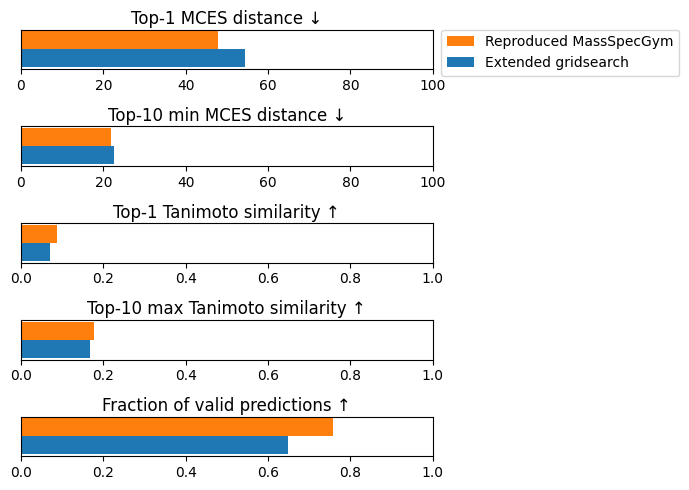
\includegraphics[width=0.6\textwidth]{figures/results/gridsearch_vs_paper.png}
    \caption{Performance comparison between the retrained SMILES model from the MassSpecGym paper versus the lowest validation loss SMILES model from the gridsearch, evaluated on the validation set}
    \label{fig:gridsearch_vs_paper}
\end{figure}

The top-1 and top-10 exact match accuracy for both models is (close to) zero.
Even though the naive sampler adds a bit of randomization by sampling from the output distribution, the retrained SMILES model from MassSpecGym outperforms the model with the lowest validation loss.

A big contributing factor to this performance difference is the fact that the retrained MassSpecGym model is able to predict 10\% more valid SMILES, as invalid SMILES have the maximum MCES distance and zero Tanimoto similarity.
The validity of the SMILES prediction relies heavily on the sampler and the temperature scaling of the output distribution.
Because only a naive sampler with no temperature scaling was used it is possible that better performance can be extracted from these models using different samplers and temperature scaling.


\section{Samplers benchmark}

To measure the influence of temperature scaling and using different samplers, and determine if these can heavily impact model performance, different samplers were used to predict the validation set of the model with the lowest loss from table \ref{tab:gridsearch}.
For this and all further experiments conducted in this thesis, the Tanimoto similarity is directly correlated to the MCES distance and will thus not be shown in the plots.
All performance differences shown with the MCES distance always show the same relative tanimoto similarities.

To measure how much the randomization of the naive sampler influences the performance of the predictions,
figure \ref{fig:naive_and_greedy} shows the 

\begin{figure}[h]
    \centering
    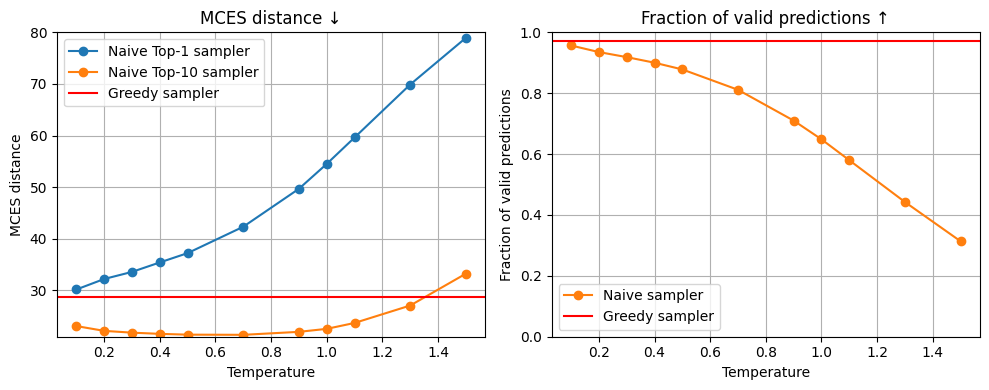
\includegraphics[width=1.0\textwidth]{figures/results/samplers/naive_and_greedy.png}
    \caption{Evaluation of the naive and greedy sampler on the validation set}
    \label{fig:naive_and_greedy}
\end{figure}



\section{\ac{BPE} as pretraining}


\section{Augmentation}

\subsection{SMILES augmentation}

\subsection{Spectral augmentation}


\section{Molecular representations benchmark}